\begin{frame}{}
    \LARGE NLP: \textbf{Long Short-Term Memory (LSTM)}
\end{frame}

\begin{frame}[allowframebreaks]{LSTM: Overview}
    \begin{itemize}
        \item LSTM is a type of RNN designed to overcome the vanishing gradient problem.
        \item It uses a memory cell to maintain information over long periods.
        \item Learns when to remember and when to forget.
        \item \textbf{Basic anatomy:}
        \begin{itemize}
            \item A cell state
            \item A hidden state
            \item Multiple gates
        \end{itemize}
        \item LSTM has three gates: input gate, forget gate, and output gate.
        \item Gates allow gradients to avoid vanishing and exploding.
    \end{itemize}
\end{frame}

\begin{frame}{LSTMs: Based on Previous Understanding}
    \begin{figure}
        \centering
        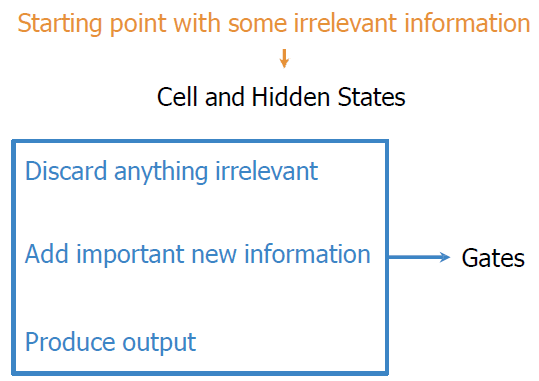
\includegraphics[width=\linewidth, height=0.9\textheight,keepaspectratio]{images/nlp/lstm-previous.png}
    \end{figure}
\end{frame}

\begin{frame}{Gates in LSTM}
    \begin{figure}
        \centering
        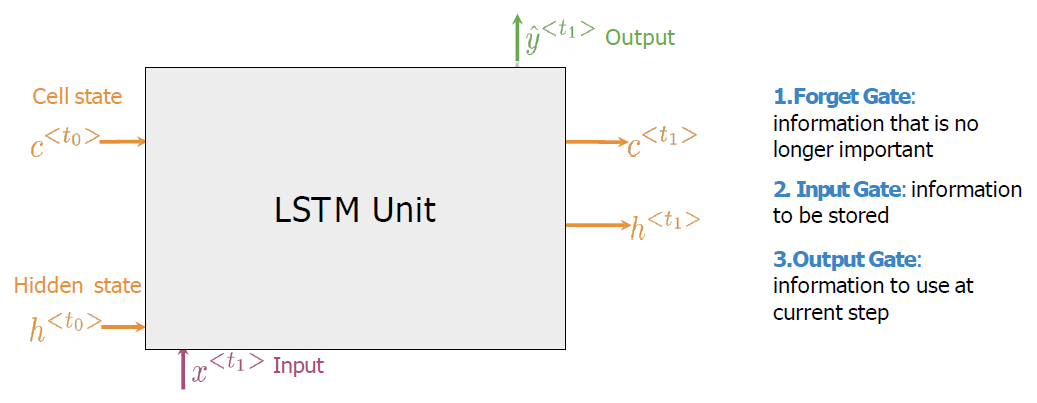
\includegraphics[width=\linewidth, height=0.9\textheight,keepaspectratio]{images/nlp/lstm-gates.png}
    \end{figure}
\end{frame}

\begin{frame}{Applications of LSTMs}
    \begin{figure}
        \centering
        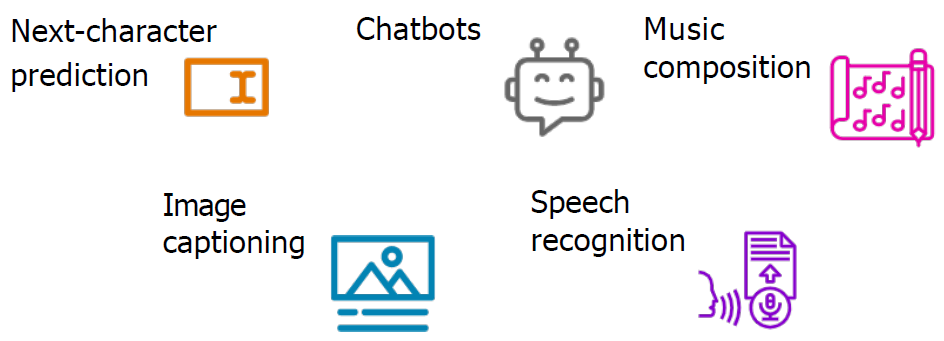
\includegraphics[width=\linewidth, height=0.9\textheight,keepaspectratio]{images/nlp/lstm-application.png}
    \end{figure}
\end{frame}